\label{es314}
\begin{flushleft}
In entrambi i casi abbiamo usato la matrice $A\in M^{3\times 3}$ con elementi:
\[ 
A =
\begin{pmatrix}
    15  & -3 &  2 \\
   -4  &  9  &  2 \\
    6  &  0  &  10 \\
\end{pmatrix}
\]
e il vettore dei termini noti $b\in \mathbb{R}^3$ con valori:
\[
{b} = (3.2, 2.3, 3.1)^T
\]
Usando il codice MatLab sottostante è possibile risolvere questi 2 esempi:
\newpage
\lstinputlisting[language=Matlab]{cap_3/es14/es14.m}
Il codice sopra restituisce l'output:
\begin{figure}[h]
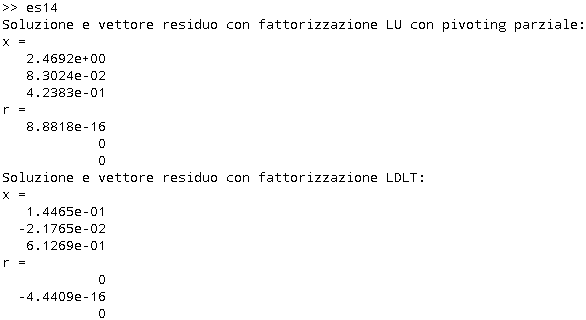
\includegraphics[left, width=400px]{cap_3/es14/es314.png}
\end{figure}
La soluzione ottenuta 
\end{flushleft}